% Teaching loop: abstract update, no implied convergence guarantee.
\documentclass[tikz,border=0pt]{standalone}
\def\FigureLanguage{en}
% Input after documentclass, before begin{document}; XeLaTeX/LuaLaTeX.
% Authors may define the Figure*Font commands before input to override defaults.
% English-only documents can set FigureLanguage=en without loading CJK support.
\providecommand{\FigureLanguage}{zh}
\providecommand{\FigurePrimary}{zh}
\makeatletter
\@ifundefined{ifFigureEnglishOnly}{%
  \newif\ifFigureEnglishOnly
  \def\FigureFontEnglishMode{en}%
  \edef\FigureFontSelectedMode{\FigureLanguage}%
  \ifx\FigureFontSelectedMode\FigureFontEnglishMode\FigureEnglishOnlytrue\fi
}{}
\makeatother
\providecommand{\FigureCJKFont}{SimSun}
\providecommand{\FigureLatinFont}{Times New Roman}
\providecommand{\FigureMathFont}{TeX Gyre Termes Math}
\ifFigureEnglishOnly
  \usepackage{fontspec}
  \typeout{FIGURE-CJK-FONT: not requested (English-only)}
\else
  \usepackage[UTF8,fontset=none]{ctex}
\fi
\usepackage{amsmath}
\usepackage{unicode-math}
\ifFigureEnglishOnly\else
\IfFontExistsTF{\FigureCJKFont}
  {\setCJKmainfont{\FigureCJKFont}\typeout{FIGURE-CJK-FONT: \FigureCJKFont}}
  {\setCJKmainfont{FandolSong-Regular}
   \typeout{FIGURE-CJK-FONT: FandolSong-Regular (fallback)}
   \PackageWarningNoLine{paperfigure}{Chinese font fallback: FandolSong-Regular}}
\fi
\IfFontExistsTF{\FigureLatinFont}
  {\setmainfont{\FigureLatinFont}\typeout{FIGURE-LATIN-FONT: \FigureLatinFont}}
  {\setmainfont{Latin Modern Roman}
   \typeout{FIGURE-LATIN-FONT: Latin Modern Roman (fallback)}
   \PackageWarningNoLine{paperfigure}{Latin font fallback: Latin Modern Roman}}
\IfFontExistsTF{\FigureMathFont}
  {\setmathfont{\FigureMathFont}\typeout{FIGURE-MATH-FONT: \FigureMathFont}}
  {\setmathfont{latinmodern-math.otf}
   \typeout{FIGURE-MATH-FONT: Latin Modern Math (fallback)}
   \PackageWarningNoLine{paperfigure}{Requested math font unavailable; using Latin Modern Math}}
% For individual bold letters/Greek symbols, not a replacement for bold equations.
% symbf follows bold-style; use symbfup/symbfit for explicit upright/italic.
\providecommand{\FigureBoldSymbol}[1]{\symbf{#1}}

\usetikzlibrary{arrows.meta,shapes.geometric}
\begin{document}
\fontsize{9.5}{11.8}\selectfont
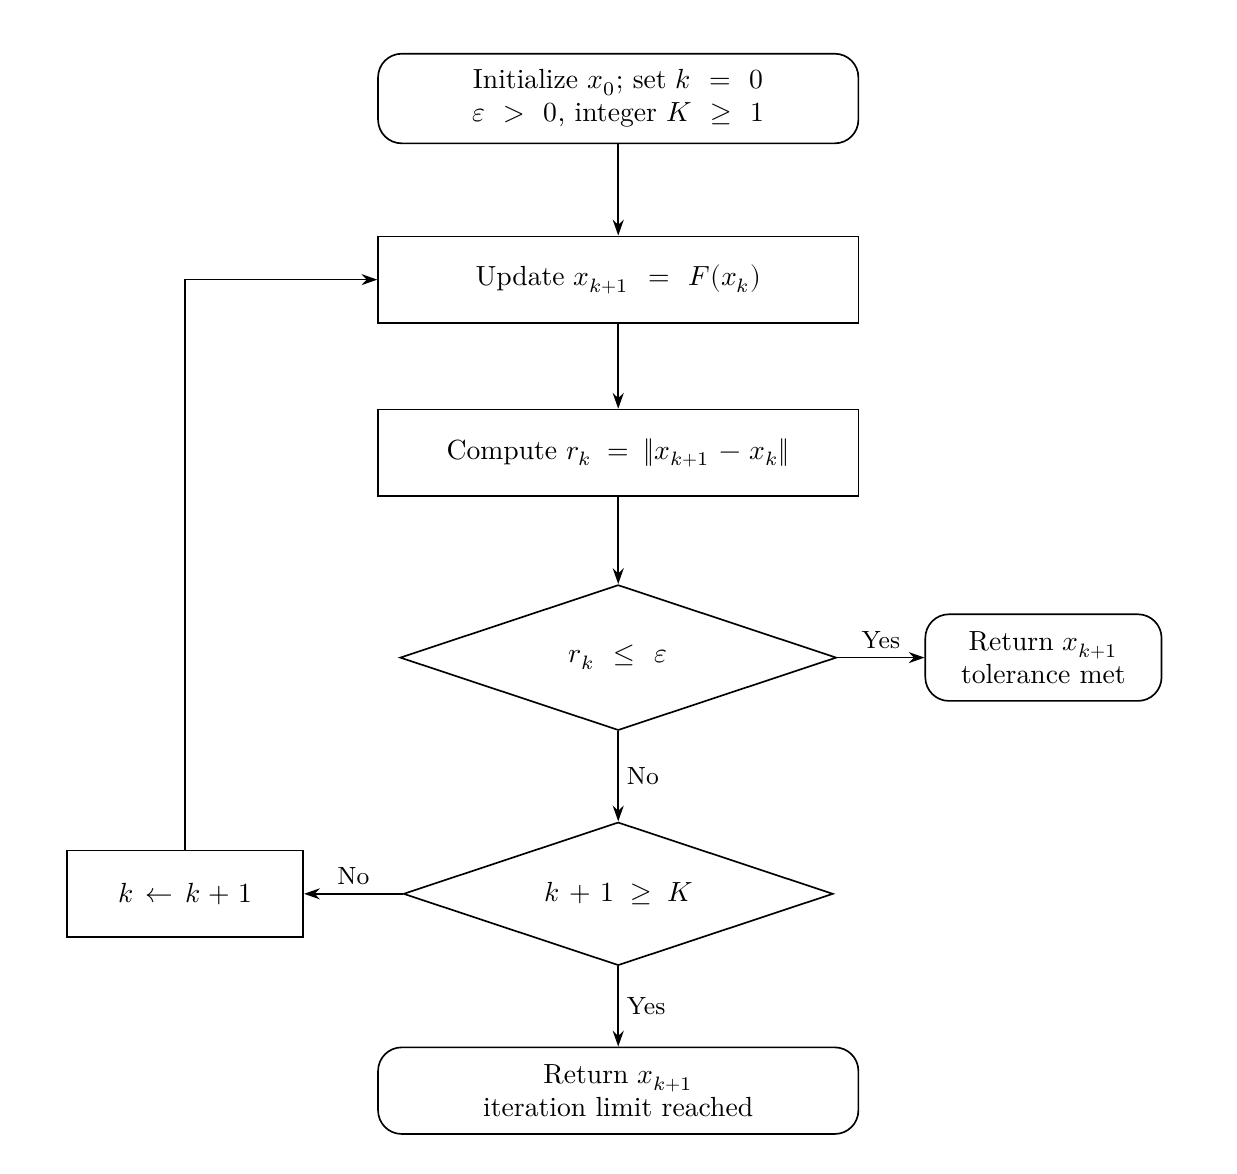
\begin{tikzpicture}[x=1mm,y=-1mm,line width=.6pt,
  >={Stealth[length=2mm,width=1.4mm]},
  box/.style={draw,rectangle,align=center,text width=57mm,minimum height=11mm,inner sep=2mm},
  term/.style={box,rounded corners=3mm},
  decide/.style={draw,diamond,aspect=3,align=center,inner sep=1.5mm,text width=34mm},
  cond/.style={fill=white,inner sep=1mm,font=\fontsize{9}{11}\selectfont}]
\path[use as bounding box] (0,0) rectangle (150,142);
\node[term] (start) at (75,9) {Initialize $x_0$; set $k=0$\\$\varepsilon>0$, integer $K\geq 1$};
\node[box] (update) at (75,32) {Update $x_{k+1}=F(x_k)$};
\node[box] (residual) at (75,54) {Compute $r_k=\lVert x_{k+1}-x_k\rVert$};
\node[decide] (stop) at (75,80) {$r_k\leq\varepsilon$};
\node[decide] (limit) at (75,110) {$k+1\geq K$};
\node[box,text width=26mm] (increment) at (20,110) {$k\leftarrow k+1$};
\node[term,text width=26mm] (converged) at (129,80) {Return $x_{k+1}$\\tolerance met};
\node[term] (budget) at (75,135) {Return $x_{k+1}$\\iteration limit reached};
\draw[->] (start) -- (update);
\draw[->] (update) -- (residual);
\draw[->] (residual) -- (stop);
\draw[->] (stop.east) -- node[cond,above]{Yes} (converged.west);
\draw[->] (stop.south) -- node[cond,right]{No} (limit.north);
\draw[->] (limit.south) -- node[cond,right]{Yes} (budget.north);
\draw[->] (limit.west) -- node[cond,above]{No} (increment.east);
\draw[->] (increment.north) |- (update.west);
\end{tikzpicture}
\end{document}
